\chapter{A look into models with dynamic ${IP_3}$}

An avenue for further work from this project is to derive a model with an ODE for dynamic $IP_3$ concentration, as suggested in Chapter 5. \citeA{sneyd} produced experimental data to prove that dynamic $IP_3$ is necessary in models for $Ca^{2+}$ signalling in airway smooth muscle cells and pancreatic acinar cells. They also derived two models with $IP_3$ as a dynamic variable.  

In \citeA{sneyd}, an experiment was carried out where a artificial pulse of $IP_3$ is applied to two different types of cells. The results from the experiment on airway smooth muscle (ASM) showed that $Ca^{2+}$ oscillations were present with constant $IP_3$, and the extra pulse increased the frequency of oscillations. In pancreatic acinar cells (PAC), it was evident that the $IP_3$ concentration was oscillating. Once the pulse was added, $IP_3$ then lay outside the oscillatory range and there was a phase lag as the concentration of $IP_3$ decreased. \citeA{sneyd} studied a total of 13 different models and chose to illustrate their experimental results using the models of \citeA{atri} and \citeA{lirinzel}. Both the Atri model and Li-Rinzel model assume $IP_3$ concentration to be constant, and thus is a parameter in the system of equations. In both models, $Ca^{2+}$ activates and inactivates the $IP_3R$, and the steady state of which follows the usual bell-shaped curve as a function of $Ca^{2+}$. A third equation for $IP_3$ is used to extend both the Atri and Li-Rinzel models. \\

\subsection*{An adapted Atri model with dynamic $IP_3$:}\\
Let us first look at how the paper by \citeA{sneyd} extends the \citeA{atri} model. The equations (\ref{origatri1st}) and (\ref{origatri2nd}) are adjusted slightly to be as in equations (\ref{sneydatri1st}) and (\ref{sneydatri2nd}) below. An equation for $Ca^{2+}$ in the ER is incorporated (shown in equation (\ref{sneydatri3rd})), as well as an equation for $IP_3$ (shown in equation (\ref{sneydatri4th})). We can see that the $IP_3$ concentration is modulated by $Ca^{2+}$. The model is defined by
\begin{align}
    \frac{dc}{dt}=& J_{channel}- J_{pump}+\delta (J_{in}- J_{pm}),\label{sneydatri1st}\\
    \tau_n\frac{dn}{dt} =& \frac{K_{inh}^2}{K_{inh}^2+c^2} -n,\label{sneydatri2nd}\\
    \gamma \frac{dc_e}{dt}=& -(J_{channel}- J_{pump}),\label{sneydatri3rd}\\
    \frac{dp}{dt}=&v_4\left(\frac{c+(1-\alpha)k_4}{c+k_4}\right)-\beta _{osc}p+s(t).\label{sneydatri4th}
\end{align}
Fluxes are given by
\begin{align}\nonumber
    J_{channel}&=k_{flux}\left(\frac{p+\mu_0K_{IP_3}}{K_{IP_3}+p}\right)n\left(\frac{K_{act}b+c}{K_{act}+c}\right)(c_e-c),\\
    J_{pump}&=\frac{V_e c}{K_e+c},\nonumber\\
    J_{in}&=\alpha_1+\alpha_2v_4,\nonumber\\
    J_{pm}&=\frac{V_pc^2}{K_p^2+c^2}.\nonumber
\end{align}


Parameter descriptions and values are given in Table \ref{sneydatritable}. Few parameter values have been adjusted from the Atri model. The leakage term, $J_{leakage}$, is now a more complex function dependent on cytosolic $Ca^{2+}$. The variable $c_e$, for $Ca^{2+}$ in the ER, allows a coupling between equations (\ref{sneydatri1st}) and (\ref{sneydatri3rd}). Equation (\ref{sneydatri4th}) is an $IP_3$ production term (dependent on $Ca^{2+}$), a degradation term for $IP_3$, and a source term, $s(t)$. The source term was present as a product of Heaviside step functions to model a pulse of $IP_3$ being added and causing a phase delay. The parameter $\gamma$ is used to adjust the amplitude of the ER $Ca^{2+}$ oscillations, as we know it is oscillating very slightly in comparison, and is passive.

Figure \ref{sneydatri2} shows a plot of equations (\ref{sneydatri1st})-(\ref{sneydatri4th}). We can see that $Ca^{2+}$ in the ER has a very small amplitude in the oscillations. Therefore, for simplicity in the model one can eliminate equation (\ref{sneydatri3rd}) and consider $Ca^{2+}$ in the ER to be constant. Once eliminated, ER $Ca^{2+}$ can be taken as a value $14 \mu M$. Now, since this is an order of magnitude greater than the range at which cytosolic $Ca^{2+}$ oscillates, the term $(c_e-c)$ is actually doing very little in contribution to the system. It can just be taken as $c_e$ on its own, which is a factor. When $Ca^{2+}$ in the ER is taken as constant, we get a decoupling with the equation (\ref{sneydatri1st}). The plot for this be seen in Figure \ref{sneydatri2}. 

\begin{figure}[!htb]
\centering
\minipage{0.8\textwidth}
  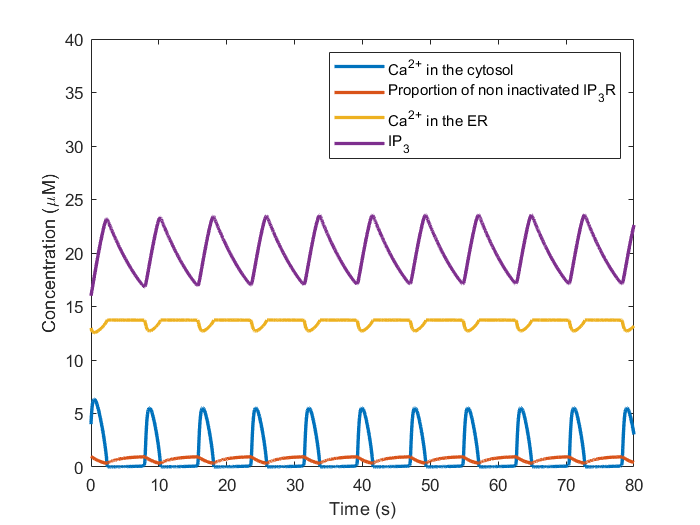
\includegraphics[width=\linewidth]{Chapters/7_appendix_A/extras/sneydatri2.png}
\endminipage\hfill\\
\minipage{0.8\textwidth}
  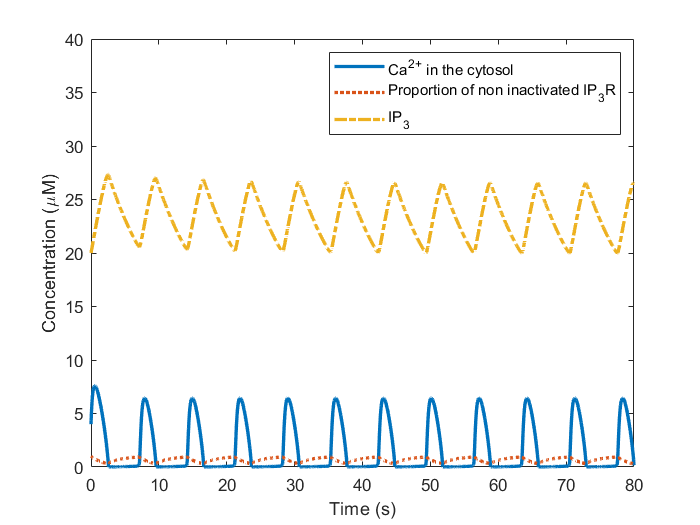
\includegraphics[width=\linewidth]{Chapters/7_appendix_A/extras/sneydatri2NOER.png}
\endminipage\hfill
\caption{The first graph shows $Ca^{2+}$ and $IP_3$ oscillations arising as solutions of the equations (\ref{sneydatri1st})-\eqref{sneydatri4th}. The second graph shows $Ca^{2+}$ and $IP_3$ oscillations arising as solutions of the  equations (\ref{sneydatri1st}), (\ref{sneydatri2nd}) and (\ref{sneydatri4th}) \cite{sneyd}. Equation (\ref{sneydatri3rd}) for the $Ca^{2+}$ concentration in the ER, $c_e$, has been omitted and $c_e$  was set to $14 \mu M$. Other parameters are taken as in Table \ref{sneydatritable}. \textit{Software:} MATLAB.}\label{sneydatri2}
\end{figure}

{The model by \citeA{sneyd} is still based on the older data \shortcite{parysetal} that the Atri model was based on, and so it does not incorporate the more accurate data on the $IP_3R$ dynamics obtained by \shortciteA{Mak1998}. } The \citeA{sneyd} model is one that should be taken into careful consideration for further work on the new model we have derived. It would be insightful to see how an $IP_3$ equation of this kind would work in a system with the $IP_3R$ dynamics from \citeA{Mak1998} incorporated. 

A similar model was derived in the paper by adding the same ODE for $IP_3$ to the Li-Rinzel model. However, with this addition came the decision to consider $n$ as a constant. This is not so relevant to our model as the fact our new model works on a gating system is crucial for the inclusion of the equation for $P_O$ \eqref{foskett}.

The third model we took a look at with dynamic $IP_3$ concentration was by \citeA{hofer}. The model presented was based around \citeA{lirinzel}, \citeA{lyttonetal}, and \citeA{carmelloetal}. It is a system of four variables with cytosolic $Ca^{2+}$ concentration, $Ca^{2+}$ concentration in the ER, cytosolic $IP_3$ concentration, and the proportion of $IP_3R$ that have not been inactivated by $Ca^{2+}$. The model assumes the $IP_3$ concentration to be highly dynamic, with oscillations in line with $Ca^{2+}$ oscillations. They show that there is both positive and negative feedback of $Ca^{2+}$, and that $IP_3$ metabolism could mediate fluctuations in $IP_3$.

The model presented accounts for the $Ca^{2+}$ fluxes across the ER and plasma membrane, the $IP_3R$ dynamics, and the formation and degradation of $IP_3$. The model is as follows.
\begin{align}
    \frac{dc}{dt}&=J_{channel}-J_{pump}+J_{leak},\\
    \frac{dc_e}{dt}&=\frac{1}{\beta}(-J_{channel}+J_{pump}),\\
    \tau_n\frac{dn}{dt}&=1-n\frac{K_{inh}+c}{K_{inh}},\\
    \tau_p\frac{dp}{dt}&=v_{PLC}-v_{deg},
\end{align}
where
\begin{align}
    J_{channel}=&\left(v_1\left(n\frac{c}{K_{act}+c}\frac{p}{K_{IP_3}+p}\right)^3+\epsilon\right)(c_e-c),\nonumber\\
    J_{pump}=&\frac{V_ec^2}{K_e^2+c^2},\nonumber\\
    J_{leak}=&v_{in}-v_{out}\nonumber\\
    =&\epsilon \left(v_0+\Phi V_{PLC}-V_{p}\frac{c^2}{K_{p}^2+c^2}\right),\nonumber\\
    v_{PLC}=&\frac{c^2}{K_{PLC}^2+c^2},\nonumber\\
    v_{deg}=&\left(k_{5P}+k_{3K}\frac{c^2}{K_{3K}^2+c^2}\right).\nonumber
\end{align}
Here we can see that $Ca^{2+}$ flux through the $IP_3R$, $J_{channel}$, is modelled based on the \citeA{lirinzel} model, that we have studied in Chapter 2. The SERCA pumps, $J_{pump}$, however, follows the model given in \citeA{lyttonetal}, and $v_{out}$ follows that in \citeA{carmelloetal}. The term $J_{pump}$ is modelled with a Hill coefficient of $2$, in contrast to $1$ in both the Atri and Li-Rinzel models. It is important that future models respect the data and consider a Hill coefficient of $2$. $Ca^{2+}$ influx, $v_{in}$, represents a leak into the cell as well as a stimulation dependent influx. The parameter $\epsilon$ is a dimensionless constant that controls the relative strength of the cell plasma membrane's fluxes. This flux is cell type specific, or in an isolated egg, non-existent.

$PLC$ produces $IP_3$ and depends on agonist dose and $Ca^{2+}$. $PLC_{\beta}$'s sensitivity towards $Ca^{2+}$ is modelled by $v_{PLC}$. Within this, $V_{PLC}$ depends on agonist concentration, and $K_{PLC}$ characterizes the sensitivity of $PLC$ to $Ca^{2+}$. $IP_3$ degradation happens through phosphorylation by $IP_3P$ and phosphorylation by $IP_3K$, which is modelled by $v_{deg}$. Respectively, $k_{5P}$ and $k_{3K}$ are the $IP_3$ dephosphorylation and phosphorylation rate constants. The $Ca^{2+}$ dependence of the $IP_3K$ is described by a Hill function with half-saturation constant $K_{3K}$. Here, the model assumes that the two enzymes are not saturated with $IP_3$, so a linear rate law in $p$ is given. This assumption is based on the work of \citeA{finketal} and \citeA{simsandallbritton}.

The modelling of the $IP_3$ equation in this paper has been well thought out, and should be considered in any future models. The Hill equation in $v_{deg}$ is a necessary component in any future model that assumes a dynamic $IP_3$ concentration. It is agreed that $IP_3$ production is catalyzed by phosphoinositide-specfic phospholipase C isoforms ($PLC$), which are activated by $Ca^{2+}$. Furthermore, $IP_3$ levels fall by dephosphorylation through $IP_3 5$-phosphatase. However, $IP_3$ degradation also happens by phosphorylation through $IP_3 3-$kinase ($IP_3K$). This is activated by $Ca^{2+}$, and hence in a mathematical model would need to show dependence on $Ca^{2+}$ \cite{hofer}.
